% Options for packages loaded elsewhere
\PassOptionsToPackage{unicode}{hyperref}
\PassOptionsToPackage{hyphens}{url}
%
\documentclass[
  twocolumn]{article}
\usepackage{amsmath,amssymb}
\usepackage{iftex}
\ifPDFTeX
  \usepackage[T1]{fontenc}
  \usepackage[utf8]{inputenc}
  \usepackage{textcomp} % provide euro and other symbols
\else % if luatex or xetex
  \usepackage{unicode-math} % this also loads fontspec
  \defaultfontfeatures{Scale=MatchLowercase}
  \defaultfontfeatures[\rmfamily]{Ligatures=TeX,Scale=1}
\fi
\usepackage{lmodern}
\ifPDFTeX\else
  % xetex/luatex font selection
\fi
% Use upquote if available, for straight quotes in verbatim environments
\IfFileExists{upquote.sty}{\usepackage{upquote}}{}
\IfFileExists{microtype.sty}{% use microtype if available
  \usepackage[]{microtype}
  \UseMicrotypeSet[protrusion]{basicmath} % disable protrusion for tt fonts
}{}
\makeatletter
\@ifundefined{KOMAClassName}{% if non-KOMA class
  \IfFileExists{parskip.sty}{%
    \usepackage{parskip}
  }{% else
    \setlength{\parindent}{0pt}
    \setlength{\parskip}{6pt plus 2pt minus 1pt}}
}{% if KOMA class
  \KOMAoptions{parskip=half}}
\makeatother
\usepackage{xcolor}
\usepackage[margin=0.95in]{geometry}
\usepackage{color}
\usepackage{fancyvrb}
\newcommand{\VerbBar}{|}
\newcommand{\VERB}{\Verb[commandchars=\\\{\}]}
\DefineVerbatimEnvironment{Highlighting}{Verbatim}{commandchars=\\\{\}}
% Add ',fontsize=\small' for more characters per line
\usepackage{framed}
\definecolor{shadecolor}{RGB}{248,248,248}
\newenvironment{Shaded}{\begin{snugshade}}{\end{snugshade}}
\newcommand{\AlertTok}[1]{\textcolor[rgb]{0.94,0.16,0.16}{#1}}
\newcommand{\AnnotationTok}[1]{\textcolor[rgb]{0.56,0.35,0.01}{\textbf{\textit{#1}}}}
\newcommand{\AttributeTok}[1]{\textcolor[rgb]{0.13,0.29,0.53}{#1}}
\newcommand{\BaseNTok}[1]{\textcolor[rgb]{0.00,0.00,0.81}{#1}}
\newcommand{\BuiltInTok}[1]{#1}
\newcommand{\CharTok}[1]{\textcolor[rgb]{0.31,0.60,0.02}{#1}}
\newcommand{\CommentTok}[1]{\textcolor[rgb]{0.56,0.35,0.01}{\textit{#1}}}
\newcommand{\CommentVarTok}[1]{\textcolor[rgb]{0.56,0.35,0.01}{\textbf{\textit{#1}}}}
\newcommand{\ConstantTok}[1]{\textcolor[rgb]{0.56,0.35,0.01}{#1}}
\newcommand{\ControlFlowTok}[1]{\textcolor[rgb]{0.13,0.29,0.53}{\textbf{#1}}}
\newcommand{\DataTypeTok}[1]{\textcolor[rgb]{0.13,0.29,0.53}{#1}}
\newcommand{\DecValTok}[1]{\textcolor[rgb]{0.00,0.00,0.81}{#1}}
\newcommand{\DocumentationTok}[1]{\textcolor[rgb]{0.56,0.35,0.01}{\textbf{\textit{#1}}}}
\newcommand{\ErrorTok}[1]{\textcolor[rgb]{0.64,0.00,0.00}{\textbf{#1}}}
\newcommand{\ExtensionTok}[1]{#1}
\newcommand{\FloatTok}[1]{\textcolor[rgb]{0.00,0.00,0.81}{#1}}
\newcommand{\FunctionTok}[1]{\textcolor[rgb]{0.13,0.29,0.53}{\textbf{#1}}}
\newcommand{\ImportTok}[1]{#1}
\newcommand{\InformationTok}[1]{\textcolor[rgb]{0.56,0.35,0.01}{\textbf{\textit{#1}}}}
\newcommand{\KeywordTok}[1]{\textcolor[rgb]{0.13,0.29,0.53}{\textbf{#1}}}
\newcommand{\NormalTok}[1]{#1}
\newcommand{\OperatorTok}[1]{\textcolor[rgb]{0.81,0.36,0.00}{\textbf{#1}}}
\newcommand{\OtherTok}[1]{\textcolor[rgb]{0.56,0.35,0.01}{#1}}
\newcommand{\PreprocessorTok}[1]{\textcolor[rgb]{0.56,0.35,0.01}{\textit{#1}}}
\newcommand{\RegionMarkerTok}[1]{#1}
\newcommand{\SpecialCharTok}[1]{\textcolor[rgb]{0.81,0.36,0.00}{\textbf{#1}}}
\newcommand{\SpecialStringTok}[1]{\textcolor[rgb]{0.31,0.60,0.02}{#1}}
\newcommand{\StringTok}[1]{\textcolor[rgb]{0.31,0.60,0.02}{#1}}
\newcommand{\VariableTok}[1]{\textcolor[rgb]{0.00,0.00,0.00}{#1}}
\newcommand{\VerbatimStringTok}[1]{\textcolor[rgb]{0.31,0.60,0.02}{#1}}
\newcommand{\WarningTok}[1]{\textcolor[rgb]{0.56,0.35,0.01}{\textbf{\textit{#1}}}}
\usepackage{longtable,booktabs,array}
\usepackage{calc} % for calculating minipage widths
% Correct order of tables after \paragraph or \subparagraph
\usepackage{etoolbox}
\makeatletter
\patchcmd\longtable{\par}{\if@noskipsec\mbox{}\fi\par}{}{}
\makeatother
% Allow footnotes in longtable head/foot
\IfFileExists{footnotehyper.sty}{\usepackage{footnotehyper}}{\usepackage{footnote}}
\makesavenoteenv{longtable}
\usepackage{graphicx}
\makeatletter
\newsavebox\pandoc@box
\newcommand*\pandocbounded[1]{% scales image to fit in text height/width
  \sbox\pandoc@box{#1}%
  \Gscale@div\@tempa{\textheight}{\dimexpr\ht\pandoc@box+\dp\pandoc@box\relax}%
  \Gscale@div\@tempb{\linewidth}{\wd\pandoc@box}%
  \ifdim\@tempb\p@<\@tempa\p@\let\@tempa\@tempb\fi% select the smaller of both
  \ifdim\@tempa\p@<\p@\scalebox{\@tempa}{\usebox\pandoc@box}%
  \else\usebox{\pandoc@box}%
  \fi%
}
% Set default figure placement to htbp
\def\fps@figure{htbp}
\makeatother
\setlength{\emergencystretch}{3em} % prevent overfull lines
\providecommand{\tightlist}{%
  \setlength{\itemsep}{0pt}\setlength{\parskip}{0pt}}
\setcounter{secnumdepth}{-\maxdimen} % remove section numbering
% definitions for citeproc citations
\NewDocumentCommand\citeproctext{}{}
\NewDocumentCommand\citeproc{mm}{%
  \begingroup\def\citeproctext{#2}\cite{#1}\endgroup}
\makeatletter
 % allow citations to break across lines
 \let\@cite@ofmt\@firstofone
 % avoid brackets around text for \cite:
 \def\@biblabel#1{}
 \def\@cite#1#2{{#1\if@tempswa , #2\fi}}
\makeatother
\newlength{\cslhangindent}
\setlength{\cslhangindent}{1.5em}
\newlength{\csllabelwidth}
\setlength{\csllabelwidth}{3em}
\newenvironment{CSLReferences}[2] % #1 hanging-indent, #2 entry-spacing
 {\begin{list}{}{%
  \setlength{\itemindent}{0pt}
  \setlength{\leftmargin}{0pt}
  \setlength{\parsep}{0pt}
  % turn on hanging indent if param 1 is 1
  \ifodd #1
   \setlength{\leftmargin}{\cslhangindent}
   \setlength{\itemindent}{-1\cslhangindent}
  \fi
  % set entry spacing
  \setlength{\itemsep}{#2\baselineskip}}}
 {\end{list}}
\usepackage{calc}
\newcommand{\CSLBlock}[1]{\hfill\break\parbox[t]{\linewidth}{\strut\ignorespaces#1\strut}}
\newcommand{\CSLLeftMargin}[1]{\parbox[t]{\csllabelwidth}{\strut#1\strut}}
\newcommand{\CSLRightInline}[1]{\parbox[t]{\linewidth - \csllabelwidth}{\strut#1\strut}}
\newcommand{\CSLIndent}[1]{\hspace{\cslhangindent}#1}
\usepackage{booktabs}
\usepackage{longtable}
\usepackage{array}
\usepackage{multirow}
\usepackage{wrapfig}
\usepackage{float}
\usepackage{colortbl}
\usepackage{pdflscape}
\usepackage{tabu}
\usepackage{threeparttable}
\usepackage{threeparttablex}
\usepackage[normalem]{ulem}
\usepackage{makecell}
\usepackage{xcolor}
\usepackage{bookmark}
\IfFileExists{xurl.sty}{\usepackage{xurl}}{} % add URL line breaks if available
\urlstyle{same}
\hypersetup{
  hidelinks,
  pdfcreator={LaTeX via pandoc}}

\author{}
\date{\vspace{-2.5em}}

\begin{document}

\section{\texorpdfstring{\textit{How Normal is the Binomial?}}{}}\label{section}

Tom Stoughton, MS Candidate\footnote{Department of Biostatistics and Informatics, Colorado School of Public Health, University of Colorado Anschutz Medical Campus, Aurora, CO}

\subsection{Abstract}\label{abstract}

In 1738, Abraham de Moivre introduced in his book \emph{The doctrine of chances: or, A method of calculating the probabilities of events in play} a formulation on how the sum of terms of the Binomial (along with many other distributions) could be approximated using an exponential equation of a familiar form. Later, this equation was translated to fit the form of a Normal distribution, with the Binomial parameters \(n\) and \(p\) showing up in the Normal parameters: \(\mu = np, \sigma^2 = npq\) where \(q = 1-p\). While most textbooks and other resources provide the useful constraint that \(np\) be ``not too small'' and ``not too big'', the general rule-of-thumb for this Normal approximation to be considered ``good'' is that \(np \geq 10\) and \(nq \geq 10\). This study tests the extents of these imprecise guidelines, attempting to find more rigid constraints on what \(n\) and \(p\) must be in order to have a good approximation of the Binomial distribution with a Normal distribution. The Kullback-Leibler (KL) divergence is used to quantitatively measure the difference between Binomial and Normal samples in a simulation study, with color-coded grids visualizing results.

\emph{Keywords: Binomial, Normal, simulation, Kullback-Leibler, approximation}

\subsection{Introduction}\label{introduction}

Approximating the Binomial distribution with the Normal has long been a staple of statistical pedagogy and applied inference, yet the conditions under which this approximation holds are often left vague. Textbooks typically assert that when both \(np\) and \(nq\) exceed 10, the Binomial can be considered approximately Normal. However, this threshold is more heuristic than empirically derived. The Normal approximation is widely used in power calculations, inference for proportions, and even in the design of sampling procedures---contexts where understanding the boundaries of its validity is crucial.

This study re-examines those boundaries through simulation. By systematically varying \(n\) and \(p\), generating both Binomial and Normal samples with corresponding parameters, and measuring their divergence, we aim to identify more precise regions where the approximation performs well and where it breaks down.

\subsection{Motivating Problem}\label{motivating-problem}

The primary motivation for this work stems from the ambiguity of the conventional rule-of-thumb. What exactly constitutes ``large enough'' \(n\) or \(np\) for the approximation to behave acceptably? Simple visual comparisons, such as overlaid histograms, suggest that at \(np = 10\), the match between the two distributions is tenuous at best. Increasing \(n\) improves smoothness, but it remains unclear whether this alone guarantees a good fit, especially for extreme \(p\) values near 0 or 1.

In exploratory plots, even with \(n=10,000\), the approximation only appears visually satisfactory when \(np > 100\). For smaller \(np\) values, discrepancies persist, particularly in the tails. These observations motivate a quantitative approach---measuring how ``Normal'' the Binomial truly is under a wide range of parameter combinations.

\subsection{Simulation Set-up}\label{simulation-set-up}

Describe your simulation study.

An example of a figure is below. In the Rmd file, the \texttt{chunk-name} can be changed to whatever you want so that it can be referenced using \texttt{\textbackslash{}ref\{tab:chunk-name\}} (where ``tab'' represents a table, ``fig'' is for a figure).

\textbf{NOTE: the code chunks have \texttt{echo=F} to suppress the code from appearing in your limited 2 page report. It can still automatically appear at the end in the appendix with a nifty line of code that appears at the end!}

\begin{figure}
\centering
\pandocbounded{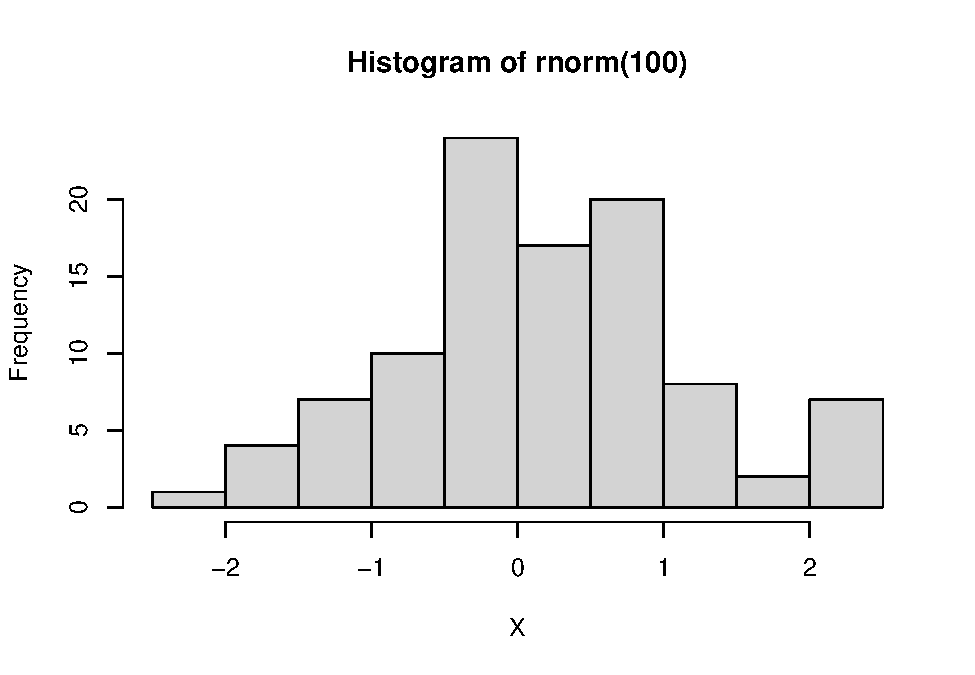
\includegraphics[keepaspectratio]{kaizer_simulation_midterm_shell_files/figure-latex/chunk-name-1.pdf}}
\caption{\label{fig:chunk-name}Caption for Figure}
\end{figure}

The code chunk(s) to implement your simulation study might be good to include at the end of this section:

\subsection{Results}\label{results}

Write your results in this section. The interpretation or implications of results will primarily appear in the following Discussion/Conclusion section.

One example you can use to create a table in our PDF output example here is with the \texttt{kableExtra} package:

\begin{table}[H]
\centering
\caption{\label{tab:result-table}Caption for table}
\centering
\begin{tabular}[t]{lcc}
\toprule
  & Column 1 of Results & Column 2 of Results\\
\midrule
Row 1 & 1 & 5\\
\cmidrule{1-3}
Row 2 & 2 & 6\\
\cmidrule{1-3}
Row 3 & 3 & 7\\
\cmidrule{1-3}
Row 4 & 4 & 8\\
\bottomrule
\end{tabular}
\end{table}

\subsection{Conclusion}\label{conclusion}

Write your conclusion here where you interpret the results for your given context, including any limitations.

\newpage
\onecolumn

\subsection{References}\label{references}

\vspace{2mm}

\phantomsection\label{refs}
\begin{CSLReferences}{0}{1}
\end{CSLReferences}

\subsection{Code Appendix}\label{code-appendix}

\begin{Shaded}
\begin{Highlighting}[]
\NormalTok{knitr}\SpecialCharTok{::}\NormalTok{opts\_chunk}\SpecialCharTok{$}\FunctionTok{set}\NormalTok{(}\AttributeTok{echo =} \ConstantTok{TRUE}\NormalTok{)}

\FunctionTok{library}\NormalTok{(kableExtra) }\CommentTok{\# load for tables}
\CommentTok{\# Create figure to demonstrate something graphically}

\FunctionTok{set.seed}\NormalTok{(}\DecValTok{515}\NormalTok{) }\CommentTok{\# set seed to reproduce example figure}
\FunctionTok{hist}\NormalTok{(}\FunctionTok{rnorm}\NormalTok{(}\DecValTok{100}\NormalTok{), }\AttributeTok{xlab=}\StringTok{\textquotesingle{}X\textquotesingle{}}\NormalTok{)}
\CommentTok{\# Implement your simulation(s) in this code chunk}

\NormalTok{mysim }\OtherTok{\textless{}{-}} \ControlFlowTok{function}\NormalTok{(x)\{}
  \CommentTok{\# function here for example}
\NormalTok{\}}

\CommentTok{\# Run simulation}
\CommentTok{\#sapply(1:1000, function(x) mysim(x))}
\CommentTok{\# Extract results for null case and scenario with expected 80\% power}
\NormalTok{tab\_res }\OtherTok{\textless{}{-}} \FunctionTok{matrix}\NormalTok{(}\DecValTok{1}\SpecialCharTok{:}\DecValTok{8}\NormalTok{, }\AttributeTok{nrow=}\DecValTok{4}\NormalTok{, }\AttributeTok{ncol=}\DecValTok{2}\NormalTok{) }\CommentTok{\# made up matrix with results}
\FunctionTok{rownames}\NormalTok{(tab\_res) }\OtherTok{\textless{}{-}} \FunctionTok{c}\NormalTok{(}\StringTok{\textquotesingle{}Row 1\textquotesingle{}}\NormalTok{,}\StringTok{\textquotesingle{}Row 2\textquotesingle{}}\NormalTok{,}\StringTok{\textquotesingle{}Row 3\textquotesingle{}}\NormalTok{,}\StringTok{\textquotesingle{}Row 4\textquotesingle{}}\NormalTok{)}

\CommentTok{\# Create table of results}
\FunctionTok{kbl}\NormalTok{(tab\_res, }
    \AttributeTok{caption =} \StringTok{\textquotesingle{}Caption for table\textquotesingle{}}\NormalTok{, }
    \AttributeTok{booktabs=}\NormalTok{T, }\AttributeTok{align=}\StringTok{\textquotesingle{}cc\textquotesingle{}}\NormalTok{,}
    \AttributeTok{col.names =} \FunctionTok{c}\NormalTok{(}\StringTok{\textquotesingle{}Column 1 of Results\textquotesingle{}}\NormalTok{,}\StringTok{\textquotesingle{}Column 2 of Results\textquotesingle{}}\NormalTok{))  }\SpecialCharTok{\%\textgreater{}\%}
    \FunctionTok{collapse\_rows}\NormalTok{(}\AttributeTok{columns=}\DecValTok{1}\NormalTok{, }\AttributeTok{latex\_hline=}\StringTok{\textquotesingle{}major\textquotesingle{}}\NormalTok{, }\AttributeTok{valign=}\StringTok{\textquotesingle{}middle\textquotesingle{}}\NormalTok{) }\SpecialCharTok{\%\textgreater{}\%}
    \FunctionTok{kable\_styling}\NormalTok{(}\AttributeTok{latex\_options =} \StringTok{"HOLD\_position"}\NormalTok{)}
\end{Highlighting}
\end{Shaded}


\end{document}
